\chapter{规范不变性与矢量势的必要性}

在开始物理内容之前，有两件实际事务。下一次课将因讲师在比利时而暂停，但课程会继续，直到十讲全部讲完。今晚的手写笔记也是在很短时间内准备好的；任何愿意为课程网站扫描这些笔记的人，都能把它们从一台慢得惊人的扫描仪中解救出来。

上一讲在数学上很密集。与其假装不是这样，我们不如把其中的核心计算再走一遍。本课程的目标是真正的理论最低限度：足以继续进入下一层次的结构。如果去掉数学而不损失物理，那就完全有理由去掉它。但精确的定律需要定量陈述，而定量陈述需要数学。记号可能会变得晦涩；这并不能证明物理学家试图用祭司般的语言把主题藏起来。

也许自然界还有一种更简单的表述尚待发现。人们可以像费曼开玩笑说的那样，把物理学的每一个方程都平方，把平方相加，再令其和等于零。这样会得到一个方程，因为每个平方都必须为零，但它不会带来任何新的理解。简单性意味着找到组织性的思想，而不只是压缩排版。当有听众反对说这样的思想必须来自某个年轻人时，这一点很容易被承认：年龄与洞见无关。

\lectureoverview{我们将首先恢复识别洛伦兹标量所需的指标记号。然后我们为相对论理论表述四条原则，完整地重复带电粒子的推导，最后两次发现规范不变性：一次作为作用量中的端点项，一次作为电磁场张量的不变性。}

\section{重访指标语言}

\subsection{为什么有些指标在上方}

设
\begin{equation}
x^\mu=(t,x,y,z),
\qquad
\mu=0,1,2,3,
\end{equation}
度规为
\begin{equation}
\eta_{\mu\nu}
=
\operatorname{diag}(-1,1,1,1).
\label{eq:sr7-metric}
\end{equation}
坐标和坐标位移被赋予上指标：
\begin{equation}
dx^\mu=(dt,dx,dy,dz).
\end{equation}
对这些坐标的导数带有下指标：
\begin{equation}
\partial_\mu
\equiv
\frac{\partial}{\partial x^\mu}.
\label{eq:sr7-gradient}
\end{equation}
哪一族称为上、哪一族称为下是一种约定，就像左和右的名称是约定一样。然而，一旦选定，这一约定就必须被一致地遵循，因为这两族的变换方式不同。

\begin{classroomqa}
\audiencequestion{一个指标什么时候应写成上标，什么时候应是下标？}
\lecturerresponse{坐标、位移以及像它们那样变换的对象被赋予上指标。导数以及像导数那样变换的对象被赋予下指标。把哪一族称为上是约定性的，但两种变换律之间的区别不是。\lecturetimestamp{00:05:03}}
\end{classroomqa}

对于标量函数 \(s(x)\)，全微分是
\begin{equation}
ds
=
\frac{\partial s}{\partial x^\mu}\,dx^\mu
=
\partial_\mu s\,dx^\mu.
\label{eq:sr7-total-differential}
\end{equation}
写开来，这就是
\begin{equation}
ds
=
\frac{\partial s}{\partial t}\,dt
+\frac{\partial s}{\partial x}\,dx
+\frac{\partial s}{\partial y}\,dy
+\frac{\partial s}{\partial z}\,dz.
\end{equation}
紧凑的表达式所说的完全相同。它不是一条新定律；它是一种装置，用来在不把四项贯穿每一行的情况下看出标量结构。

\begin{figure}[htbp]
\centering
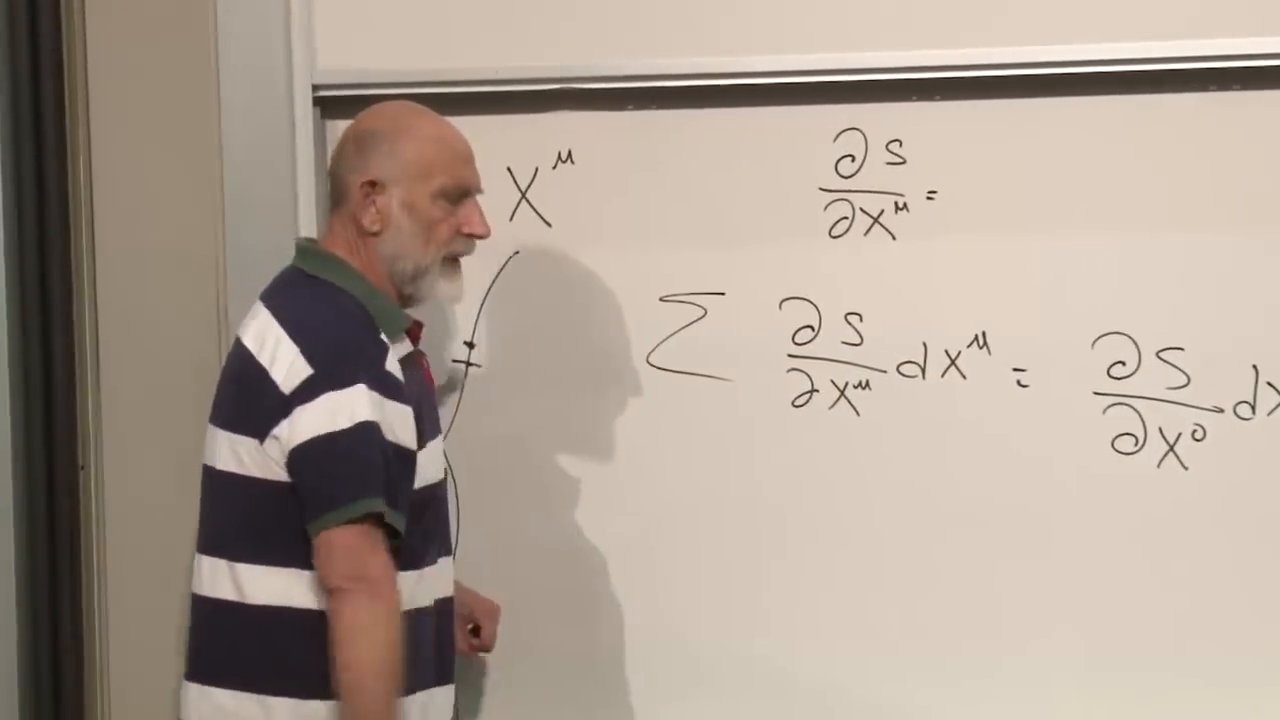
\includegraphics[width=0.90\textwidth]{lecture_07_figure_01.png}
\caption{由下指标梯度和上指标位移组装而成的标量微分。}
\lectureframe{00:08:20}
\end{figure}

爱因斯坦约定现在就很直接了：一个指标在上方出现一次、在下方出现一次，就求和。因此，\eqref{eq:sr7-total-differential} 中的缩并是一个标量。矢量和余矢量有更深的几何解释，但这一讨论推迟到广义相对论。

\subsection{升指标}

每个四维矢量都有由度规联系的上指标和下指标形式：
\begin{equation}
A_\mu=\eta_{\mu\nu}A^\nu.
\end{equation}
由 \eqref{eq:sr7-metric}，
\begin{equation}
A_0=-A^0,
\qquad
A_m=A^m,
\qquad m=1,2,3.
\label{eq:sr7-lowering}
\end{equation}
因此，升指标或降指标会改变时间分量的符号，而对空间分量不做任何改变。同样的规则适用于导数：
\begin{equation}
\begin{aligned}
\partial_\mu
&=
\left(
\frac{\partial}{\partial t},
\frac{\partial}{\partial x},
\frac{\partial}{\partial y},
\frac{\partial}{\partial z}
\right),\\[0.5em]
\partial^\mu
&=
\left(
-\frac{\partial}{\partial t},
\frac{\partial}{\partial x},
\frac{\partial}{\partial y},
\frac{\partial}{\partial z}
\right).
\end{aligned}
\label{eq:sr7-raised-gradient}
\end{equation}

\begin{figure}[htbp]
\centering
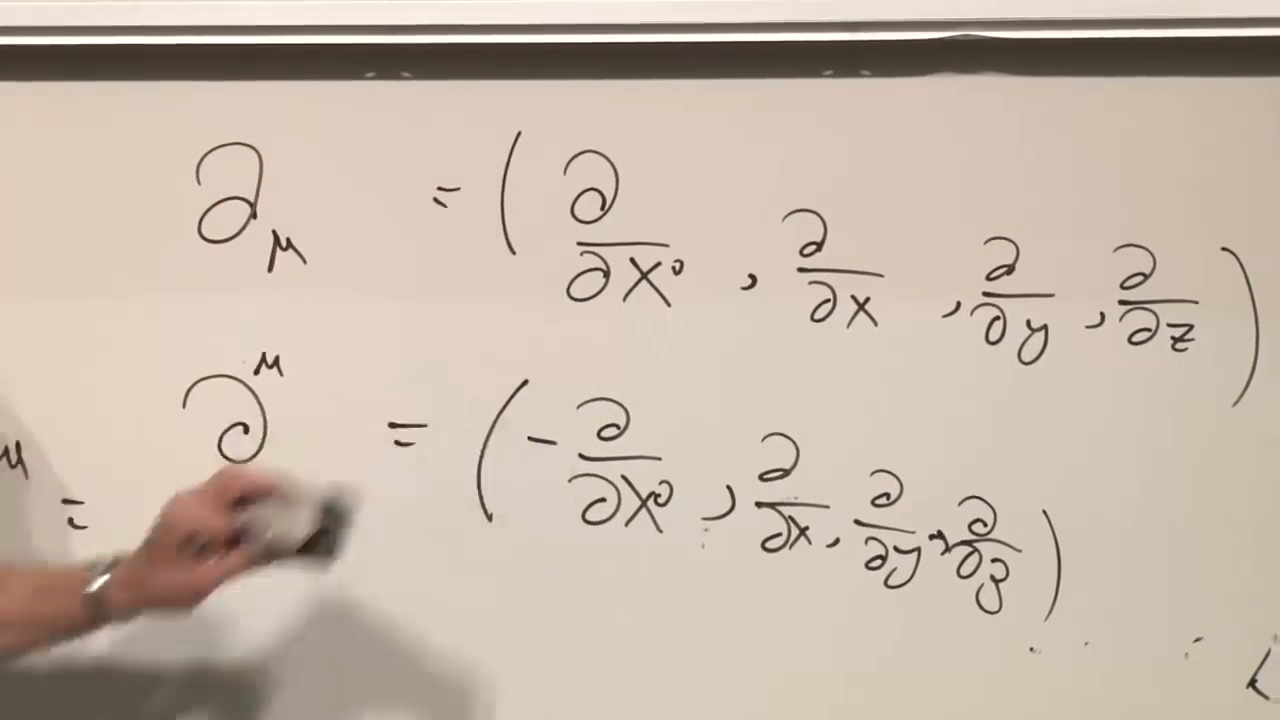
\includegraphics[width=0.90\textwidth]{lecture_07_figure_02.png}
\caption{下指标和上指标的导数算符；只有时间分量改变符号。}
\lectureframe{00:12:30}
\end{figure}

\begin{classroomqa}
\audiencequestion{偏导数是否总是带有下指标，它也能被升起来吗？}
\lecturerresponse{算符 \(\partial/\partial x^\mu\) 自然是
\(\partial_\mu\)，一个余矢量。应用度规给出
\(\partial^\mu=\eta^{\mu\nu}\partial_\nu\)；在平直时空中，这仅仅反转时间分量。\lecturetimestamp{00:11:00}}
\end{classroomqa}

不变间隔是熟悉的例子：
\begin{equation}
x_\mu x^\mu
=
x^2+y^2+z^2-t^2.
\label{eq:sr7-interval}
\end{equation}
一个上指标和一个下指标的缩并产生一个洛伦兹标量。这条简单的识别规则就是如此小心地保留这套记号的原因。

\section{构造理论的四条原则}

假设某个实验揭示了一种新现象，而我们想为它建立一套理论。有四条原则可以组织这一探索。它们最终可能需要被修正，但现今每一个成功的基础理论都符合它们的模式。

\subsection{作用量原理}

第一项要求是作用量。对于粒子力学，
\begin{equation}
I[x]
=
\int dt\,L(x,\dot x),
\label{eq:sr7-particle-action-general}
\end{equation}
而物理路径在保持其端点固定的变分下是稳定的：
\begin{equation}
\delta I=0.
\end{equation}
由此得到的方程是
\begin{equation}
\frac{d}{dt}
\left(
\frac{\partial L}{\partial\dot x^m}
\right)
=
\frac{\partial L}{\partial x^m}.
\label{eq:sr7-EL}
\end{equation}

作用量原理并非美学上的装饰。它是将对称性与守恒律联系起来的框架。作用量的时间平移对称性给出能量守恒；空间平移给出动量守恒；相关的对称性构成其他守恒量的基础。仅有作用量并不等于守恒律，但它是使对称性成为守恒律的结构。

\subsection{局域性}

第二项要求是局域性。如果小提琴弦上的某一点受到扰动，相邻的一段会首先响应。再相邻的一段接着响应，扰动便传播开来。其效应最终可以到达整条弦，但短时间内的直接影响是局域的。

对于粒子，局域性由沿轨迹求值的拉格朗日量来体现。它依赖于同一时刻的位置和速度，而不依赖于任意一对相隔遥远的时间。对于场\(\phi(x)\)，
\begin{equation}
I[\phi]
=
\int d^4x\,
\mathcal L\!\left(\phi,\partial_\mu\phi\right).
\label{eq:sr7-local-field-action}
\end{equation}
一个事件处的密度依赖于该处的场及其一阶导数。它不包含此处的场与一个无关的远处点处的场的直接乘积。

\begin{figure}[htbp]
\centering
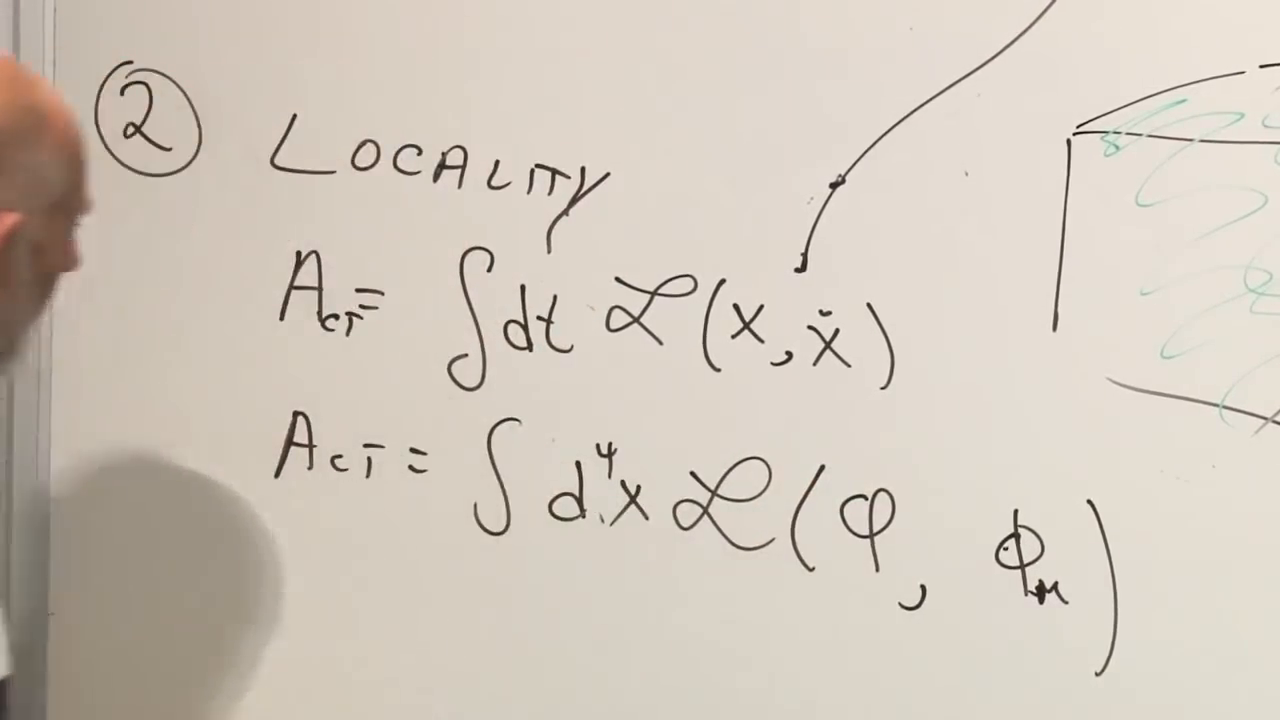
\includegraphics[width=0.90\textwidth]{lecture_07_figure_03.png}
\caption{在局域性原理下方展示的粒子与场的作用量。}
\lectureframe{00:19:30}
\end{figure}

这就是为什么局域的运动方程是微分方程。导数比较的是无穷邻近的值。非局域的替代方案可能会把现在的加速度与一个完全不同时刻的力联系起来，或者把两个遥远时刻的速度与第三个时刻的力联系起来。这样的定律在数学上可以想象，但局域性排除了它们。

\begin{classroomqa}
\audiencequestion{量子纠缠是否与这一局域性原理相矛盾？}
\lecturerresponse{在此处所使用的动力学意义上并不矛盾。纠缠产生关联，但Alice的局域操作不能用来改变Bob的约化态，也不能瞬时向他发送可控信号。抛硬币的类比隔离出了这一区别：看到一枚硬币揭示了另一个人拥有的是哪一枚相关联的硬币，但它并不作用于那枚远处的硬币。量子关联比那个经典类比更丰富，然而它们仍然不能提供超光速信号。\lecturetimestamp{00:20:02}}
\end{classroomqa}

\subsection{洛伦兹不变性}

第三项要求是定律在每个惯性系中具有相同的形式。实用的构造规则很简单：拉格朗日量必须是洛伦兹标量，这样作用量才是不变的。诸如\(\partial_\mu\phi\,\partial^\mu\phi\)这样的上--下指标缩并提供了构造的基石。

在广义相对论中，这一陈述被扩展了。被积函数是一个标量密度，不变性从洛伦兹变换扩展到任意坐标变换。这一精细化并不取代当前的原则；它是该原则在弯曲时空中的形式。

\begin{classroomqa}
\audiencequestion{洛伦兹不变性是否只是狭义相对论的一条规则，而非真正普遍的原理？}
\lecturerresponse{对于平直时空中的非引力问题，洛伦兹不变性是正确的陈述。在弯曲时空中，人们用适当的标量密度取代标量拉格朗日量，并要求在任意坐标变换下不变。除了这一精细化之外，同样的构造哲学依然成立。\lecturetimestamp{00:24:16}}
\end{classroomqa}

\begin{classroomqa}
\audiencequestion{粒子拉格朗日量和场拉格朗日密度的量纲是什么？}
\lecturerresponse{粒子拉格朗日量具有能量的量纲。在\(I=\int dt\,d^3x\,\mathcal L\)中，空间测度提供一个体积，因此\(\mathcal L\)具有单位体积能量的量纲。将其对空间积分便给出具有能量量纲的普通拉格朗日量。\lecturetimestamp{00:25:49}}
\end{classroomqa}

\subsection{规范不变性}

第四项要求是规范不变性。在这一点上，它被有意留作神秘。一位听众给出了一个有用的预期：也许人们可以向拉格朗日量中添加某些东西而不改变物理。这很接近，但“某些”这个词几乎承担了全部的工作。

\begin{figure}[htbp]
\centering
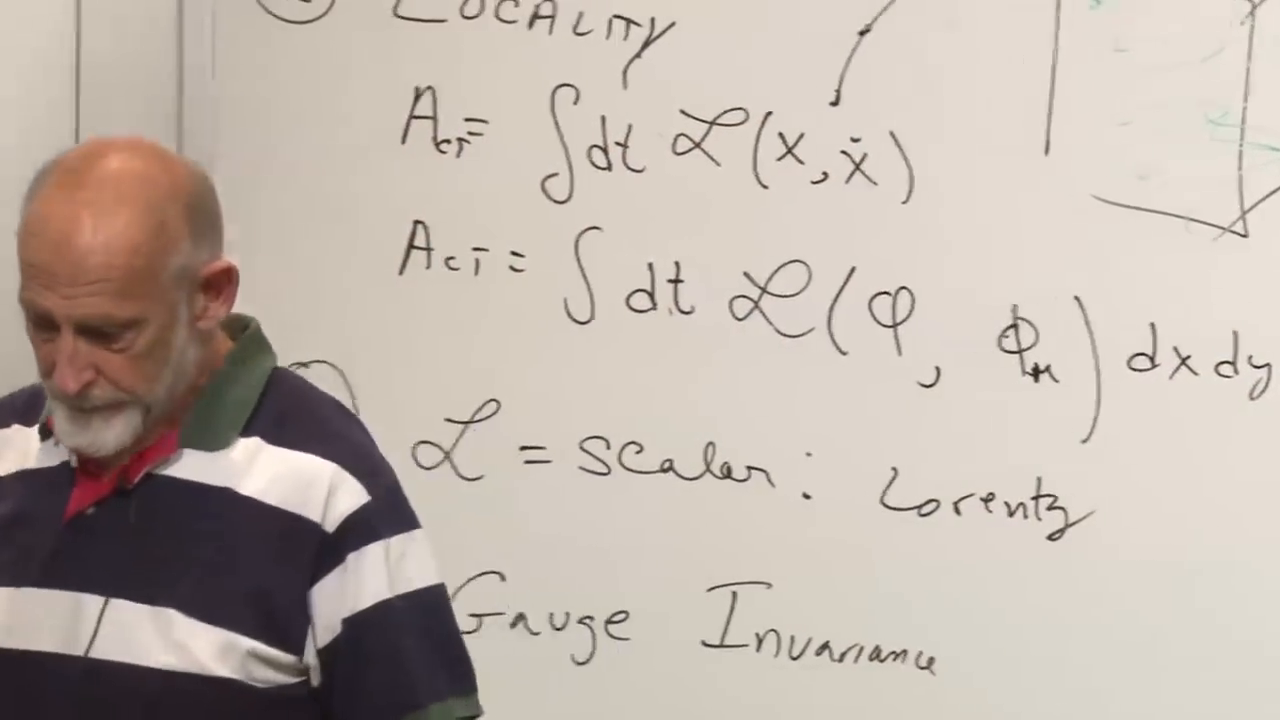
\includegraphics[width=0.90\textwidth]{lecture_07_figure_04.png}
\caption{局域性、标量构造、洛伦兹不变性和规范不变性被汇集在黑板上。}
\lectureframe{00:27:00}
\end{figure}

我们推迟给出定义，因为带电粒子的计算中已经包含了它。重复那个计算并非绕路。它将表明为什么矢量势是被强加给我们的，以及为什么一旦引入它，它就包含了一种冗余。

\section{为什么矢量势是必要的}

对于缓慢运动的带电粒子，目标方程是熟悉的洛伦兹力定律
\begin{equation}
m\mathbf a
=
e\left(
\mathbf E+\mathbf v\times\mathbf B
\right).
\label{eq:sr7-lorentz-target}
\end{equation}

\begin{figure}[htbp]
\centering
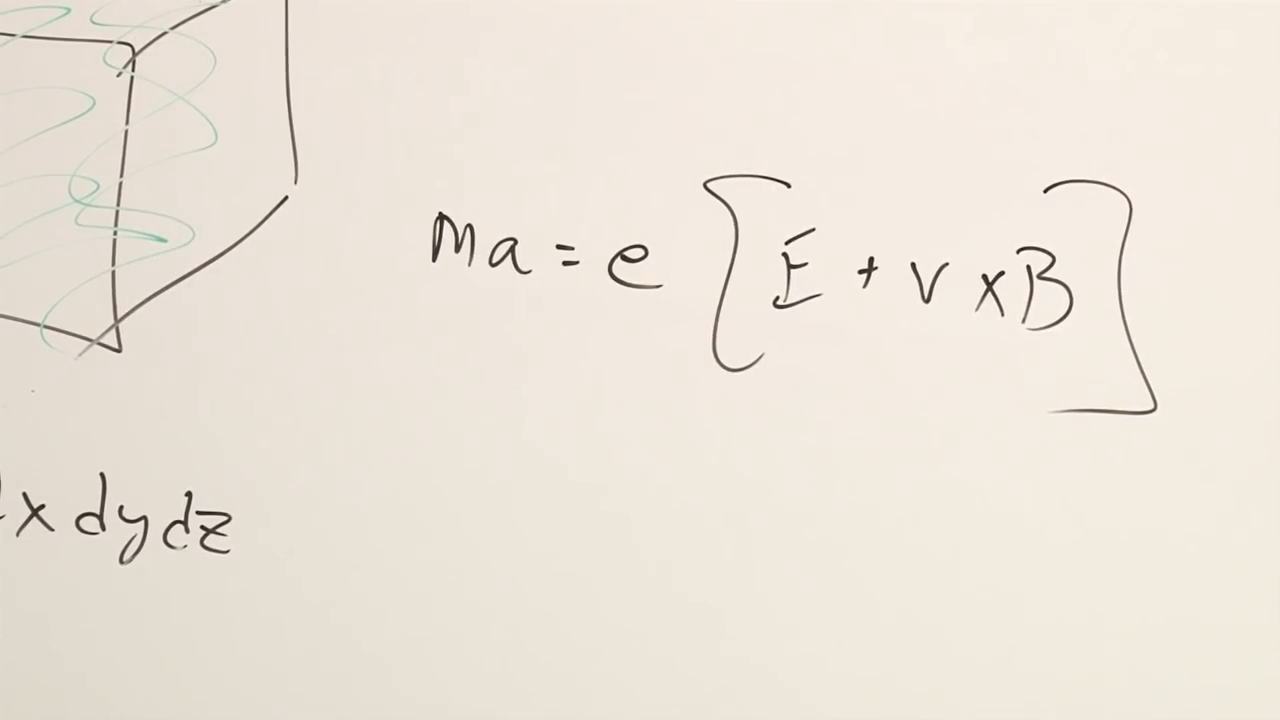
\includegraphics[width=0.90\textwidth]{lecture_07_figure_05.png}
\caption{在重新引入矢量势之前写下的熟悉的力定律。}
\lectureframe{00:29:08.870}
\end{figure}

\eqref{eq:sr7-lorentz-target}中不出现矢量势。人们可以直接用\(\mathbf E\)和\(\mathbf B\)写出运动方程。困难更具结构性：在本讲座所使用的局域性和洛伦兹不变性假设下，带电粒子的相互作用不能仅用那些场、位置和速度直接写成一个世界线作用量。需要势\(A_\mu\)来构造局域标量耦合。

\begin{classroomqa}
\audiencequestion{如果力定律已经只包含\(\mathbf E\)和\(\mathbf B\)，为什么要引入\(A_\mu\)？}
\lecturerresponse{因为运动方程还不是作用量原理。在本讲座的局域洛伦兹不变框架内，带电粒子作用量需要四维势。仅凭场可以陈述力，但势才是使力能够从一个标量世界线作用量导出的对象。\lecturetimestamp{00:29:06}}
\end{classroomqa}

\subsection{世界线作用量}

候选作用量有一个自由部分和一个相互作用部分：
\begin{equation}
I[x]
=
-m\int d\tau
-e\int A_\mu(x)\,dx^\mu.
\label{eq:sr7-worldline-action}
\end{equation}
第一项加上了轨迹每个无穷小段的固有时长度。按构造它是一个标量。在第二项中，\(A_\mu(x)\)在粒子所占据的事件处取值，并与位移\(dx^\mu\)缩并。该增量也是标量，并且沿世界线是局域的。

\begin{figure}[htbp]
\centering
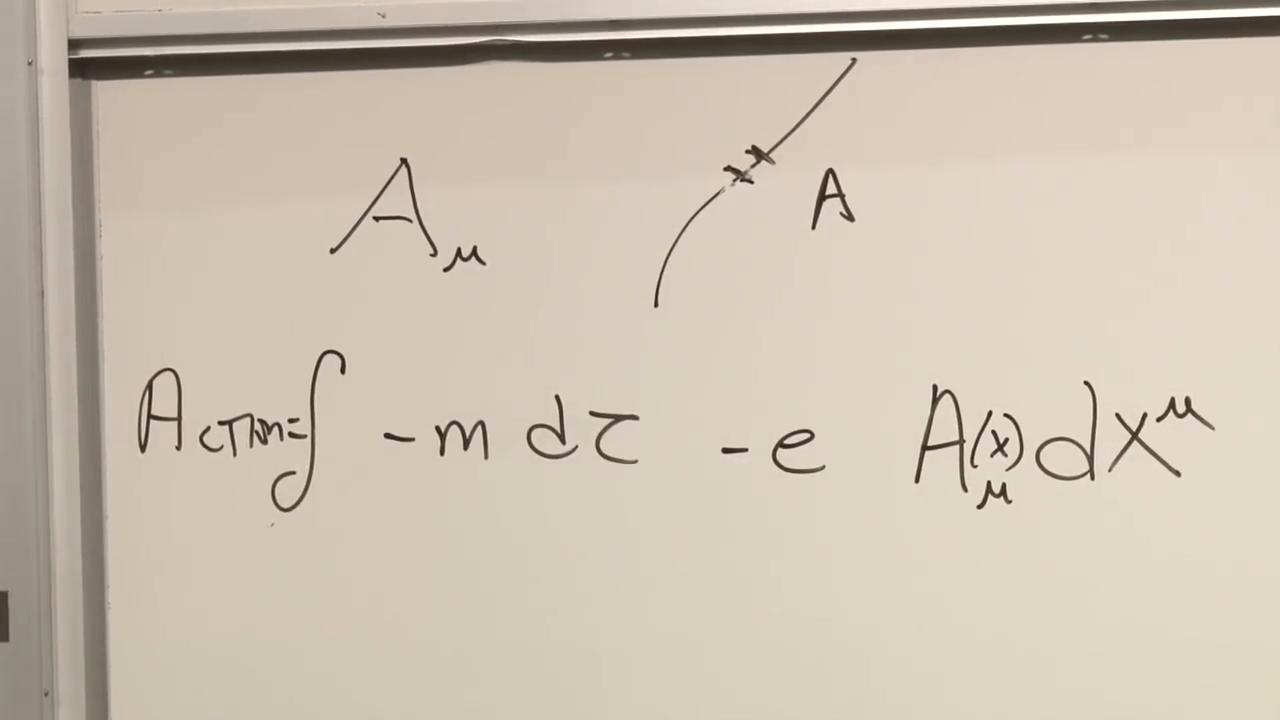
\includegraphics[width=0.90\textwidth]{lecture_07_figure_06.png}
\caption{带电粒子作用量的两部分以及局域缩并\(A_\mu(x)dx^\mu\)。}
\lectureframe{00:31:20}
\end{figure}

\subsection{将作用量改写为普通时间形式}

为了使用熟悉的欧拉--拉格朗日方程，将每个世界线增量除以\(dt\)：
\begin{equation}
\frac{d\tau}{dt}
=
\sqrt{1-\dot{\mathbf x}^{\,2}},
\qquad
\dot{\mathbf x}^{\,2}
=
\dot x^2+\dot y^2+\dot z^2.
\end{equation}
\(dx^\mu/dt\)的四个分量为
\begin{equation}
\frac{dx^\mu}{dt}
=
\left(1,\dot x,\dot y,\dot z\right).
\end{equation}
因此，
\begin{align}
I
&=
\int dt\,
\left[
-m\sqrt{1-\dot{\mathbf x}^{\,2}}
-eA_\mu\frac{dx^\mu}{dt}
\right]
\notag\\
&=
\int dt\,
\left[
-m\sqrt{1-\dot{\mathbf x}^{\,2}}
-e\left(A_0+A_m\dot x^m\right)
\right].
\label{eq:sr7-action-in-t}
\end{align}
普通时间拉格朗日量因此为
\begin{equation}
\begin{aligned}
L(x,\dot x,t)
&=
-m\sqrt{1-\dot{\mathbf x}^{\,2}}
\\
&\quad -e\left[
A_0(x,t)+A_m(x,t)\dot x^m
\right].
\end{aligned}
\label{eq:sr7-lagrangian}
\end{equation}

\begin{figure}[htbp]
\centering
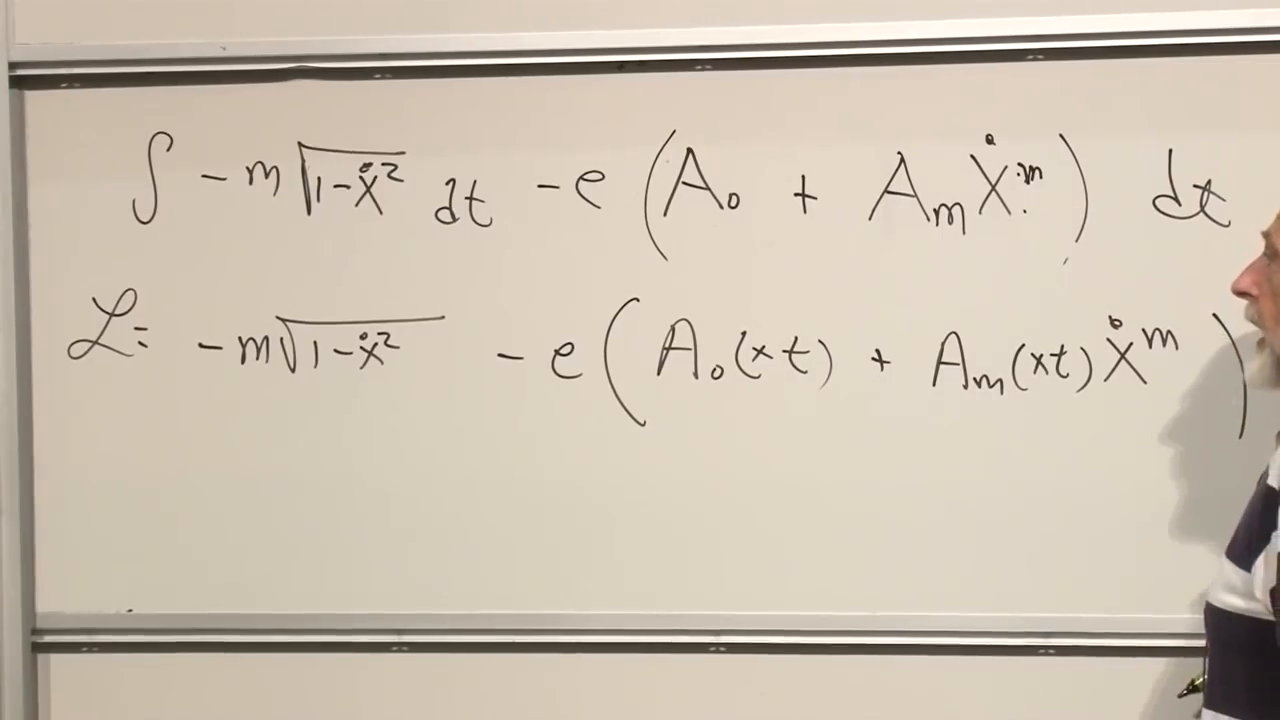
\includegraphics[width=0.90\textwidth]{lecture_07_figure_07.png}
\caption{将世界线作用量改写为普通时间积分，并从其被积函数读出拉格朗日量。}
\lectureframe{00:35:30}
\end{figure}

至此，富有想象力的部分已经结束。一旦选定了拉格朗日量，其余就是机械性的工作。这种机械性工作可能冗长而乏味，但这种乏味并非空洞：正是它揭示了电、磁和相对论结构。讲演者开玩笑说，发现原理是令人愉快的部分，而推导其全部后果则是交给研究生去做的事。

\begin{classroomqa}
\audiencequestion{在这个计算中，\(A_m\)或\(\dot x^m\)上的空间指标可以上移或下移吗？}
\lecturerresponse{可以。空间度规是单位矩阵，因此升高或降低一个拉丁指标不会改变其分量值。需要小心其符号的是时间指标。\lecturetimestamp{00:34:10}}
\end{classroomqa}

\section{欧拉--拉格朗日计算}

\subsection{正则动量与一个现场修正}

选择一个空间分量\(x^m\)。对\eqref{eq:sr7-lagrangian}的自由项求导得到
\begin{equation}
\frac{m\dot x_m}{\sqrt{1-\dot{\mathbf x}^{\,2}}}
=
m u_m,
\qquad
u^\mu\equiv\frac{dx^\mu}{d\tau}.
\end{equation}
黑板上第一次尝试到此为止。听众的修正抓住了遗漏之处：相互作用项也依赖于\(\dot x^m\)。完整的导数是
\begin{equation}
\frac{\partial L}{\partial\dot x^m}
=
\frac{m\dot x_m}{\sqrt{1-\dot{\mathbf x}^{\,2}}}
-eA_m
=
m u_m-eA_m.
\label{eq:sr7-canonical-momentum}
\end{equation}

\begin{classroomqa}
\audiencequestion{\(\partial L/\partial\dot x^m\)的第一个表达式是否遗漏了电磁项的贡献？}
\lecturerresponse{是的。将
\(-eA_n\dot x^n\)对\(\dot x^m\)求导会贡献
\(-eA_m\)。修正后的正则动量是
\(m u_m-eA_m\)，而不只是机械动量。
\lecturetimestamp{00:37:24}}
\end{classroomqa}

\begin{figure}[htbp]
\centering
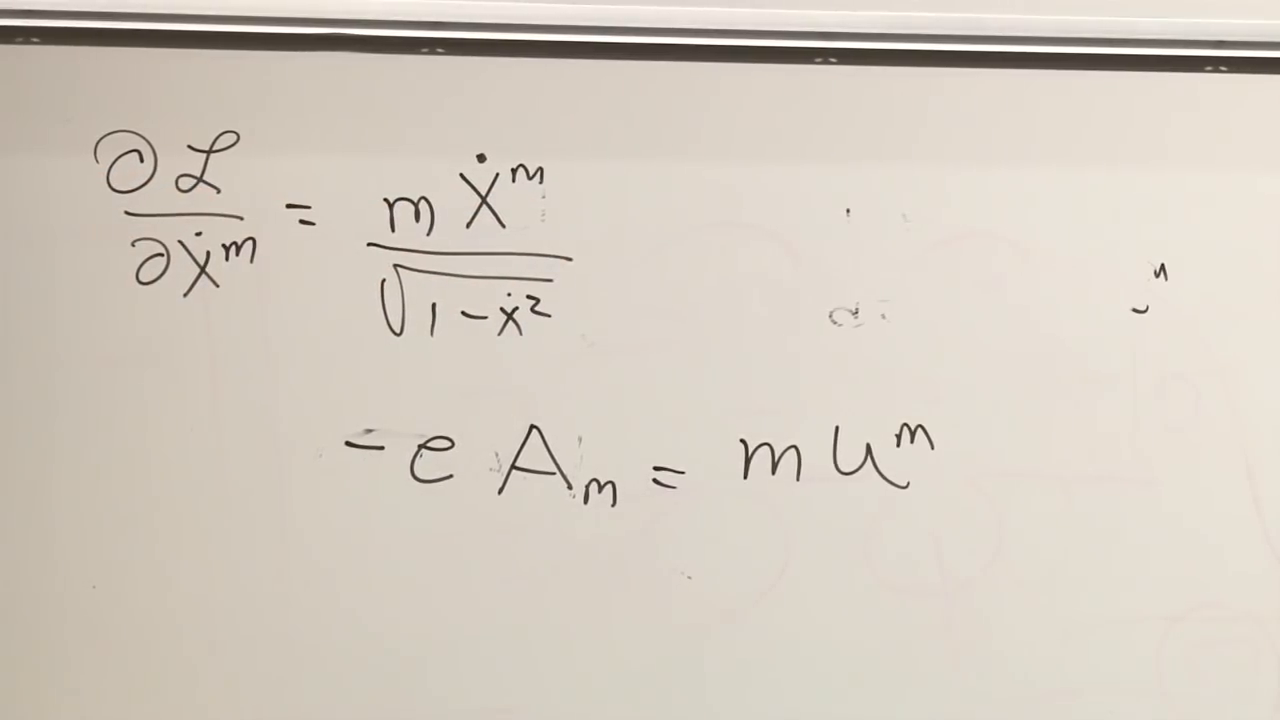
\includegraphics[width=0.90\textwidth]{lecture_07_figure_08.png}
\caption{同时包含机械项和势项的修正后正则动量。}
\lectureframe{00:38:30}
\end{figure}

\subsection{沿运动路径求导}

欧拉--拉格朗日方程的左边是
\begin{equation}
\frac{d}{dt}
\left(
\frac{\partial L}{\partial\dot x^m}
\right)
=
m\frac{du_m}{dt}
-e\frac{dA_m(x(t),t)}{dt}.
\end{equation}
势的变化有两个原因：它可能显式依赖于时间，并且粒子穿过其空间变化。链式法则给出
\begin{equation}
\frac{dA_m}{dt}
=
\partial_0A_m
+\dot x^n\partial_nA_m.
\label{eq:sr7-chain-rule}
\end{equation}
详细写来，第二项意味着
\begin{equation}
\dot x\,\frac{\partial A_m}{\partial x}
+\dot y\,\frac{\partial A_m}{\partial y}
+\dot z\,\frac{\partial A_m}{\partial z}.
\end{equation}

\begin{figure}[htbp]
\centering
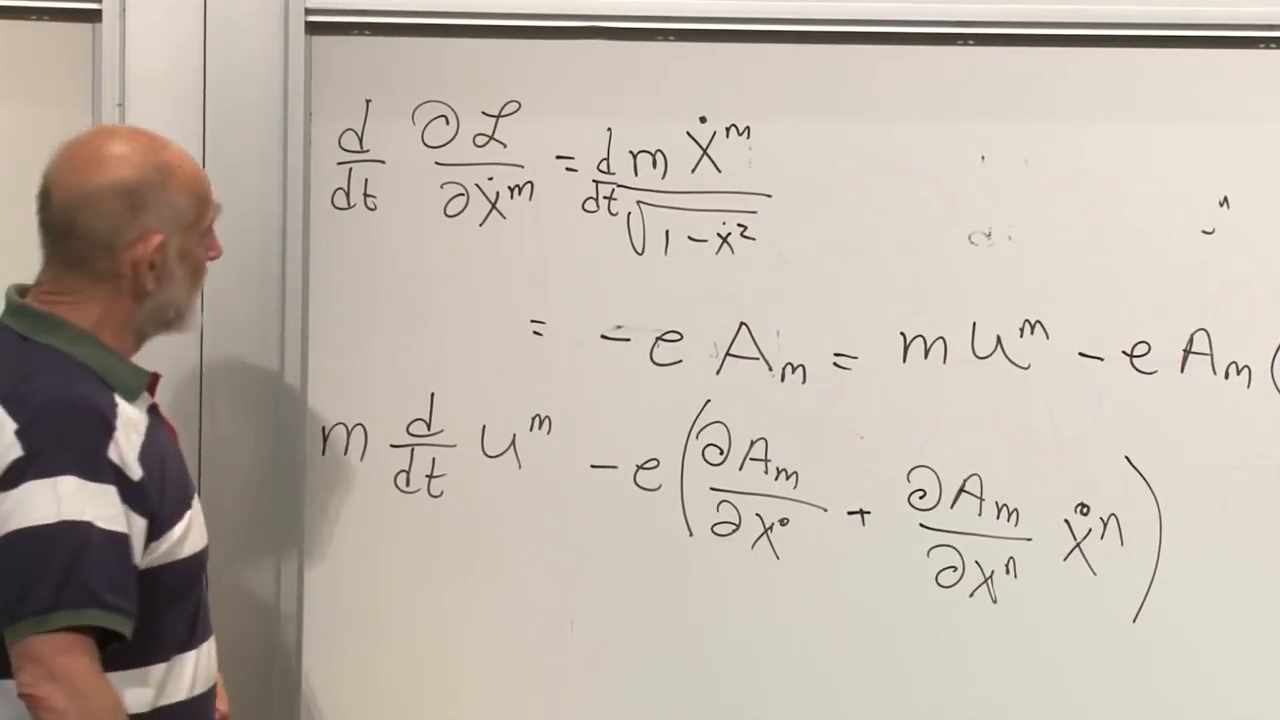
\includegraphics[width=0.90\textwidth]{lecture_07_figure_09.png}
\caption{\(A_m\)的时间导数中的显式部分和对流部分。}
\lectureframe{00:42:10}
\end{figure}

在右侧，
\begin{equation}
\frac{\partial L}{\partial x^m}
=
-e\partial_mA_0
-e\dot x^n\partial_mA_n.
\label{eq:sr7-spatial-derivative-L}
\end{equation}
自由项没有显式的位置依赖。在
\eqref{eq:sr7-spatial-derivative-L}中，\(m\)是自由指标，用于选取一个方程；\(n\)是重复的哑指标，并被求和。重命名该哑指标不会改变任何东西。正是这一区别使得讲师在合并各项之前对字母格外斟酌。

令两侧相等并整理，得到
\begin{equation}
m\frac{du_m}{dt}
=
e\left(
\partial_0A_m-\partial_mA_0
\right)
+e\dot x^n
\left(
\partial_nA_m-\partial_mA_n
\right).
\label{eq:sr7-grouped-force}
\end{equation}

\begin{figure}[htbp]
\centering
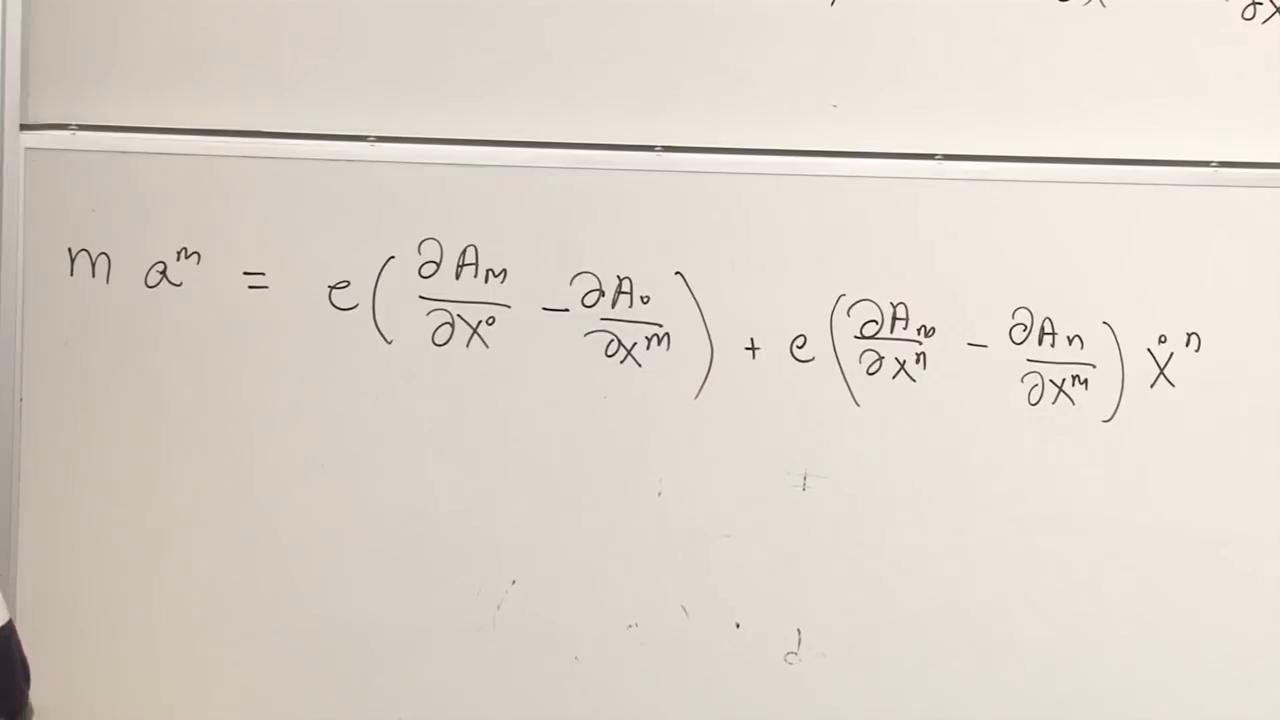
\includegraphics[width=0.90\textwidth]{lecture_07_figure_10.png}
\caption{力被分离为一个与速度无关的括号和一个速度线性的反对称括号。}
\lectureframe{00:49:30}
\end{figure}

\subsection{识别电场与磁场}

第一个括号不含粒子速度。按照本作用量的约定，定义
\begin{equation}
E_m
\equiv
\partial_0A_m-\partial_mA_0.
\label{eq:sr7-E-from-A}
\end{equation}
它恰好具有电场的作用角色。第二个括号在其空间指标上是反对称的：
\begin{equation}
C_{mn}
\equiv
\partial_nA_m-\partial_mA_n.
\label{eq:sr7-C}
\end{equation}
它的三个独立分量是空间势的旋度，其取向按讲课约定选取，使得
\begin{equation}
\dot x^n C_{mn}
=
\left(\mathbf v\times\mathbf B\right)_m.
\label{eq:sr7-magnetic-identification}
\end{equation}
详细的分量验证留作黑板上的练习。结构上的识别已经显而易见：一个矢量的反对称空间导数有三个分量，恰好是\(\mathbf B\)所携带的数目，并且它乘以速度。

\begin{figure}[htbp]
\centering
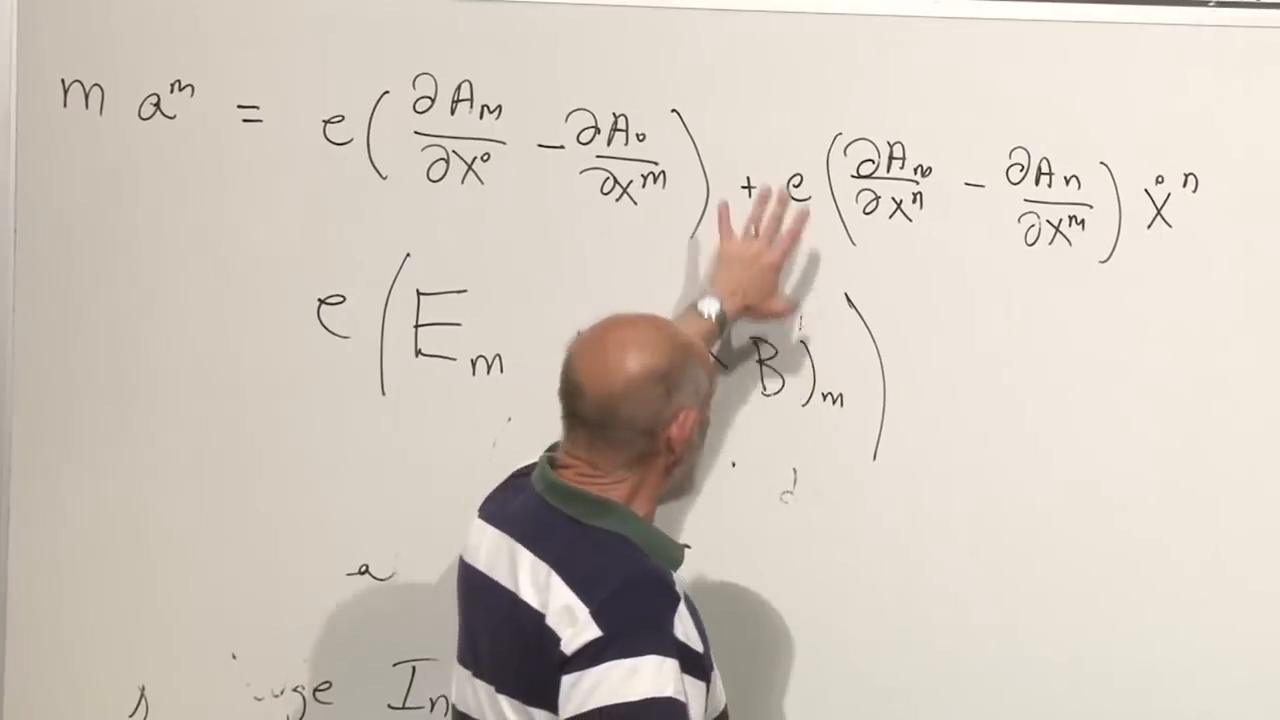
\includegraphics[width=0.90\textwidth]{lecture_07_figure_11.png}
\caption{这两个导数括号被识别为洛伦兹力的电场部分和磁场部分。}
\lectureframe{00:52:00}
\end{figure}

因此，方程\eqref{eq:sr7-grouped-force}从矢量势作用量中重新得到了洛伦兹力。它还完成了更重要的事情：它揭示出那些将被构成场张量的反对称化导数。

\section{从普通时间到四维矢量方程}

\subsection{固有时转换}

\eqref{eq:sr7-grouped-force}的左侧不是牛顿加速度\(d\mathbf v/dt\)。它是一个四维速度分量的普通时间导数：
\begin{equation}
\frac{du^m}{dt}
=
\frac{du^m}{d\tau}\frac{d\tau}{dt}.
\end{equation}
将方程乘以\(dt/d\tau\)。于是
\begin{equation}
\dot x^n\frac{dt}{d\tau}
=
\frac{dx^n}{dt}\frac{dt}{d\tau}
=
u^n,
\qquad
\frac{dt}{d\tau}=u^0.
\end{equation}
空间方程变为
\begin{align}
m\frac{du^m}{d\tau}
&=
e\left(
\partial_0A_m-\partial_mA_0
\right)u^0
\notag\\
&\quad
+e\left(
\partial_nA_m-\partial_mA_n
\right)u^n.
\label{eq:sr7-proper-spatial}
\end{align}

\begin{figure}[htbp]
\centering
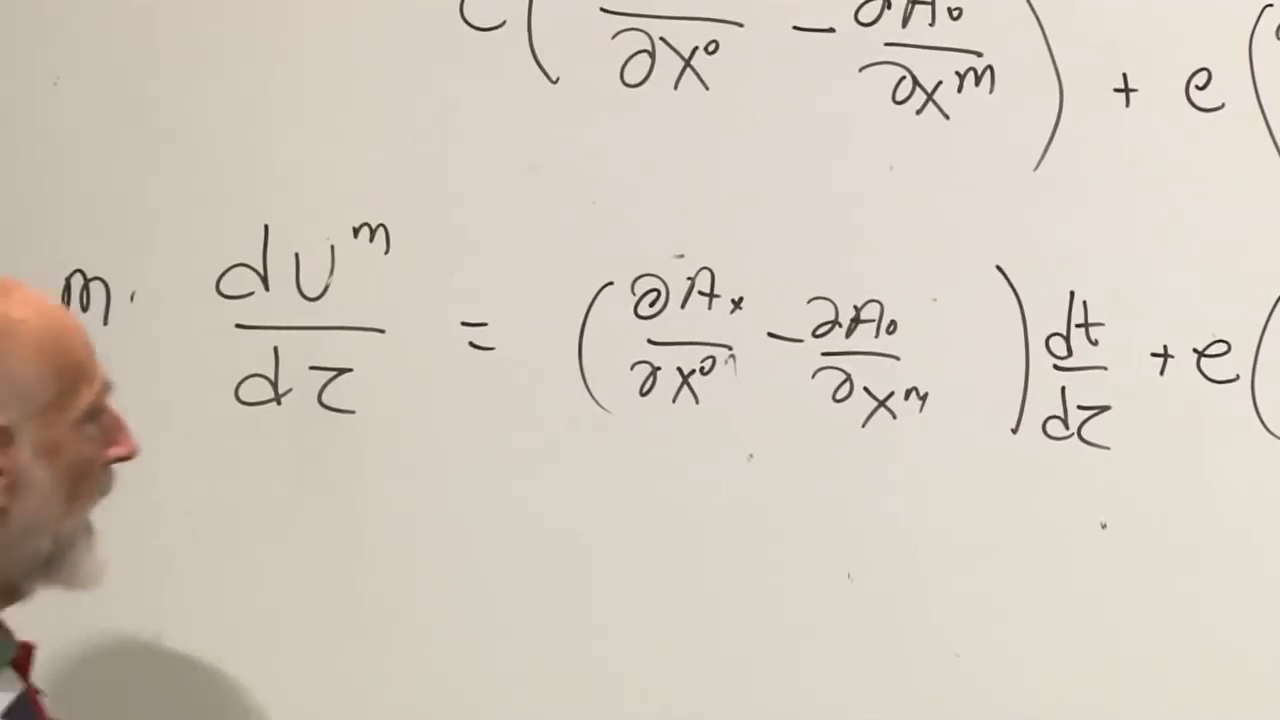
\includegraphics[width=0.90\textwidth]{lecture_07_figure_12.png}
\caption{因子\(dt/d\tau\)将普通速度转换为四维速度的分量。}
\lectureframe{00:56:30}
\end{figure}

左侧是固有加速度：
\begin{equation}
\frac{du^\mu}{d\tau}
=
\frac{d^2x^\mu}{d\tau^2}.
\end{equation}
它是一个四维矢量。因此右侧必须由一个作用于\(u^\nu\)的二阶张量组装而成。

\subsection{场张量与力定律}

选择约定
\begin{equation}
F_{\mu\nu}
\equiv
\partial_\mu A_\nu-\partial_\nu A_\mu.
\label{eq:sr7-F-definition}
\end{equation}
它是反对称的：
\begin{equation}
F_{\mu\nu}=-F_{\nu\mu}.
\end{equation}
使用\eqref{eq:sr7-worldline-action}中的相互作用符号，紧凑方程为
\begin{equation}
\boxed{
m\frac{du^\mu}{d\tau}
=
-eF^\mu{}_\nu u^\nu
}.
\label{eq:sr7-covariant-force}
\end{equation}
等价地，在命名\(F_{\mu\nu}\)之前，
\begin{equation}
m\frac{du^\mu}{d\tau}
=
e\left(
\partial_\nu A^\mu-\partial^\mu A_\nu
\right)u^\nu.
\end{equation}
不同的度规、电荷和势约定会重新分配整体符号。不变的内容是势的反对称化导数及其与四维速度的缩并。

\begin{figure}[htbp]
\centering
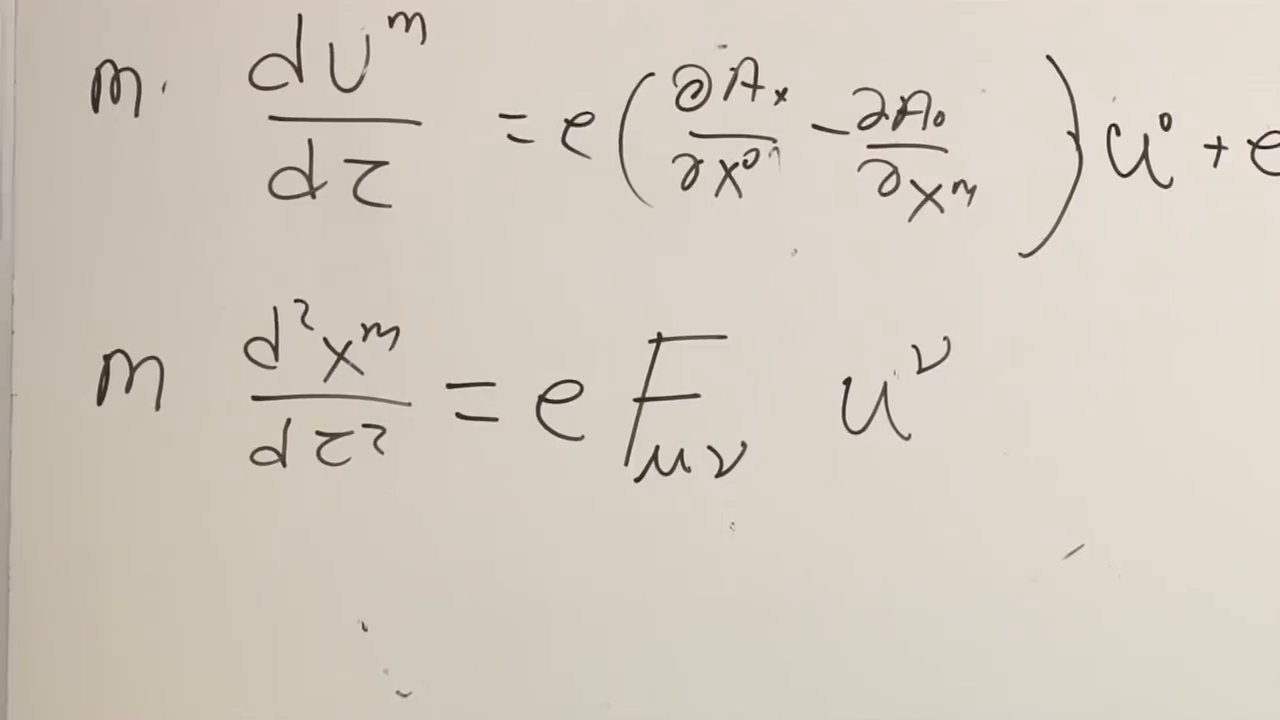
\includegraphics[width=0.90\textwidth]{lecture_07_figure_13.png}
\caption{将固有时方程打包为一个作用于四维速度的二阶场张量。}
\lectureframe{00:58:25}
\end{figure}

\begin{classroomqa}
\audiencequestion{推导产生了三个空间方程。为什么允许再添加第四个方程？}
\lecturerresponse{标量作用量保证了洛伦兹协变的结果。一旦两侧之差被识别为四维矢量，洛伦兹变换就会混合其空间分量和时间分量。一个四维矢量方程不可能自洽地只有三个分量；时间分量与空间分量相伴。\lecturetimestamp{00:59:40}}
\end{classroomqa}

\begin{classroomqa}
\audiencequestion{像\((1,2,3,4)\)这样一份固定的数字列表本身是洛伦兹不变的四维矢量吗？}
\lecturerresponse{不是。这样的数字可以在某个选定参考系中作为矢量的分量，但分量会变换。即使在二维中，分量为\((1,2)\)的矢量在旋转后的参考系中也可以描述为\((0,\sqrt5)\)。几何矢量持续存在；它的数值分量列表则不然。\lecturetimestamp{01:00:28}}
\end{classroomqa}

\begin{figure}[htbp]
\centering
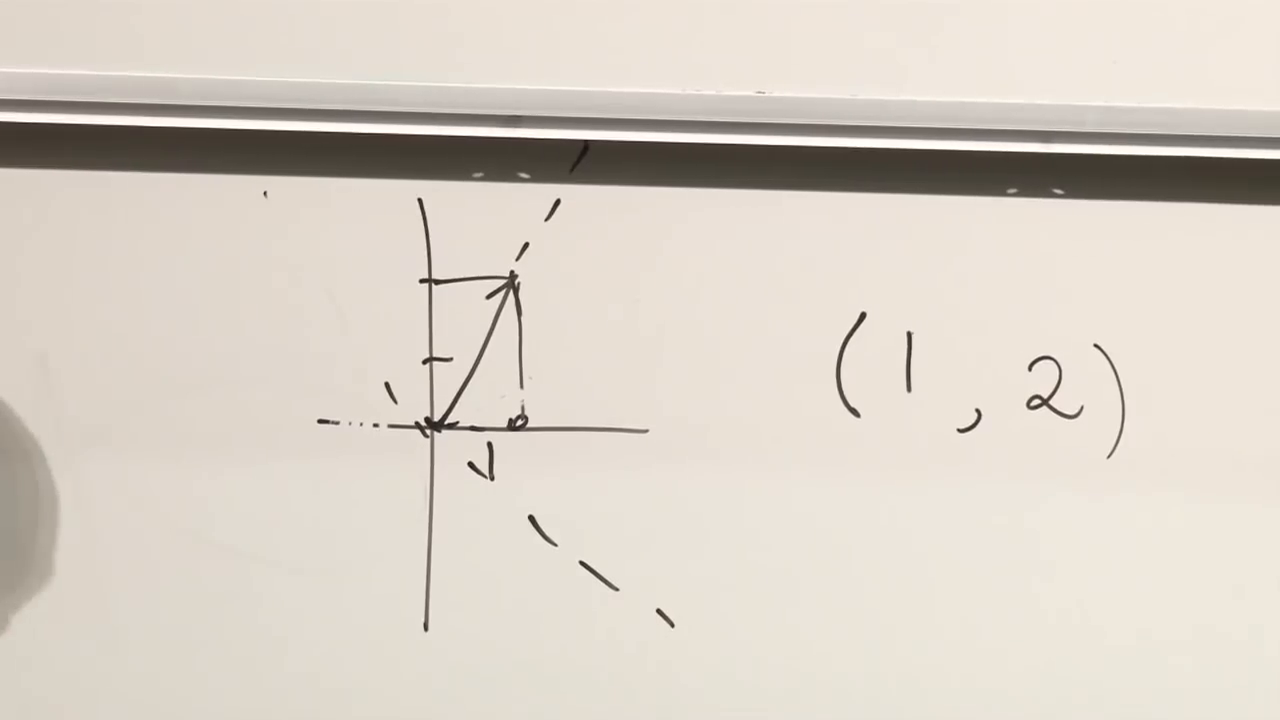
\includegraphics[width=0.90\textwidth]{lecture_07_figure_14.png}
\caption{一个二维矢量在与该矢量本身对齐的坐标轴中重新表示。}
\lectureframe{01:02:00}
\end{figure}

\begin{classroomqa}
\audiencequestion{如果目标是用固有时取代普通时间，为什么\(\partial_0A_m=\partial A_m/\partial t\)仍然出现？}
\lecturerresponse{目标并不是抹去每一个字母\(t\)。目标是用显明的四维矢量记号写出动力学。算符\(\partial_0\)是协变四维梯度的时问分量，正如\(\partial_m\)是其空间分量一样。它属于四维张量内部。\lecturetimestamp{01:05:10}}
\end{classroomqa}

讲课利用这一时刻重述局域性。局域方程将某个事件处的加速度与该事件处的场和速度联系起来。它不会把现在的加速度与某个遥远时刻的力联系起来。

\begin{figure}[htbp]
\centering
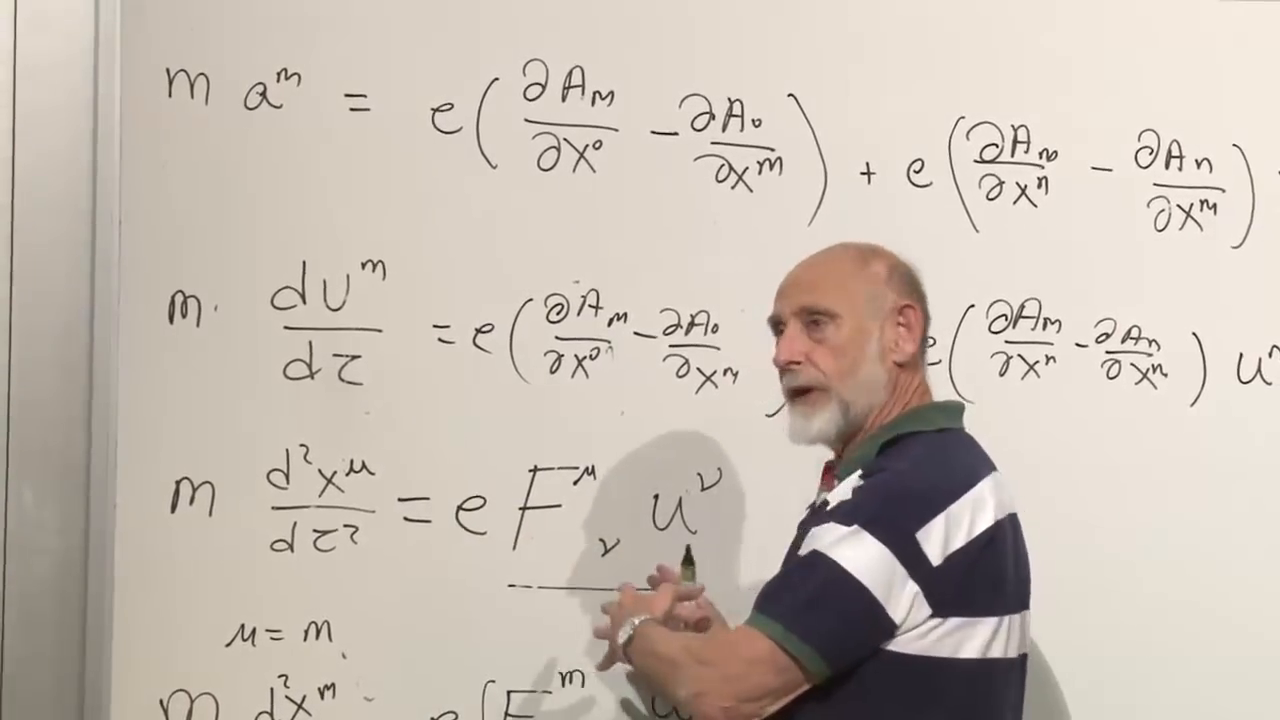
\includegraphics[width=0.90\textwidth]{lecture_07_figure_15.png}
\caption{用于将定域性重新表述为微分动力学的协变力方程。}
\lectureframe{01:05:50}
\end{figure}

\subsection{展示电磁分量}

对于全上指标张量，黑板上所用的约定给出
\begin{equation}
F^{\mu\nu}
=
\begin{pmatrix}
0&-E_x&-E_y&-E_z\\
E_x&0&B_z&-B_y\\
E_y&-B_z&0&B_x\\
E_z&B_y&-B_x&0
\end{pmatrix}.
\label{eq:sr7-F-matrix}
\end{equation}
行指标为\(\mu\)，列指标为\(\nu\)。混合的时间--空间分量包含电场；空间--空间块包含磁场。反对称性使对角线为零，并将十六个显示分量约化为六个独立分量。

\begin{figure}[htbp]
\centering
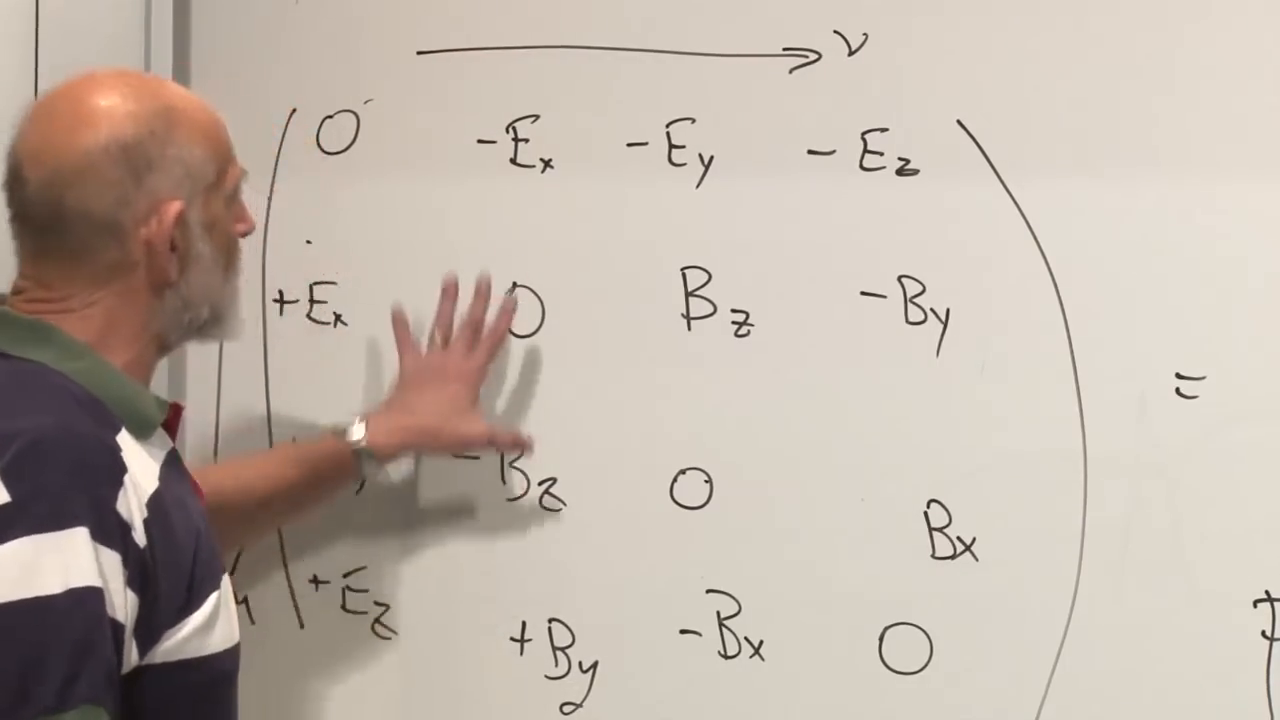
\includegraphics[width=0.90\textwidth]{lecture_07_figure_16.png}
\caption{完整的电磁张量，其中电分量位于时间--空间位置，磁分量位于空间块中。}
\lectureframe{01:12:10}
\end{figure}

\begin{classroomqa}
\audiencequestion{是否存在标准规则来决定哪个张量指标标记行、哪个标记列？}
\lecturerresponse{这是一种显示约定。这里第一个指标
\(\mu\) 沿竖直方向排列，第二个指标 \(\nu\) 沿水平方向排列。
一旦宣布了这一约定，每个分量都可以无歧义地读出。提升一个时间指标会引入一个符号，但不会改变行--列约定。\lecturetimestamp{01:09:01}}
\end{classroomqa}

\begin{classroomqa}
\audiencequestion{哪些指标位置保持反对称性？}
\lecturerresponse{张量 \(F_{\mu\nu}\) 和 \(F^{\mu\nu}\) 是反对称的。混合阵列 \(F^\mu{}_\nu\) 在普通矩阵转置下不是反对称的：提升一个时间指标会改变电分量位置，使时间--空间对成为对称的，而纯空间的磁块仍保持反对称。讲师在黑板上简要检验并否定了相反的可能性之后得出了这一结论。
\lecturetimestamp{01:13:18}}
\end{classroomqa}

\section{什么算作不变性？}

直到现在，我们才回到第四条原理。不变性是一种使运动方程保持不变的改变。作用量本身可以完全不变，也可以改变一个边界项，而该边界项对变分方程没有影响。

\subsection{无质量标量的常数平移}

考虑一维空间中的无质量标量方程，
\begin{equation}
\frac{\partial^2\phi}{\partial t^2}
-\frac{\partial^2\phi}{\partial x^2}
=0,
\label{eq:sr7-wave}
\end{equation}
它来自
\begin{equation}
\mathcal L_0
=
-\frac12\partial_\mu\phi\,\partial^\mu\phi.
\label{eq:sr7-massless-L}
\end{equation}
如果 \(\phi\) 是一个解，那么
\begin{equation}
\phi\longrightarrow\phi+c,
\label{eq:sr7-constant-shift}
\end{equation}
也是解，其中 \(c\) 是常数。\(c\) 的每个导数都为零，因此方程和仅含导数的拉格朗日量都不变。

\begin{figure}[htbp]
\centering
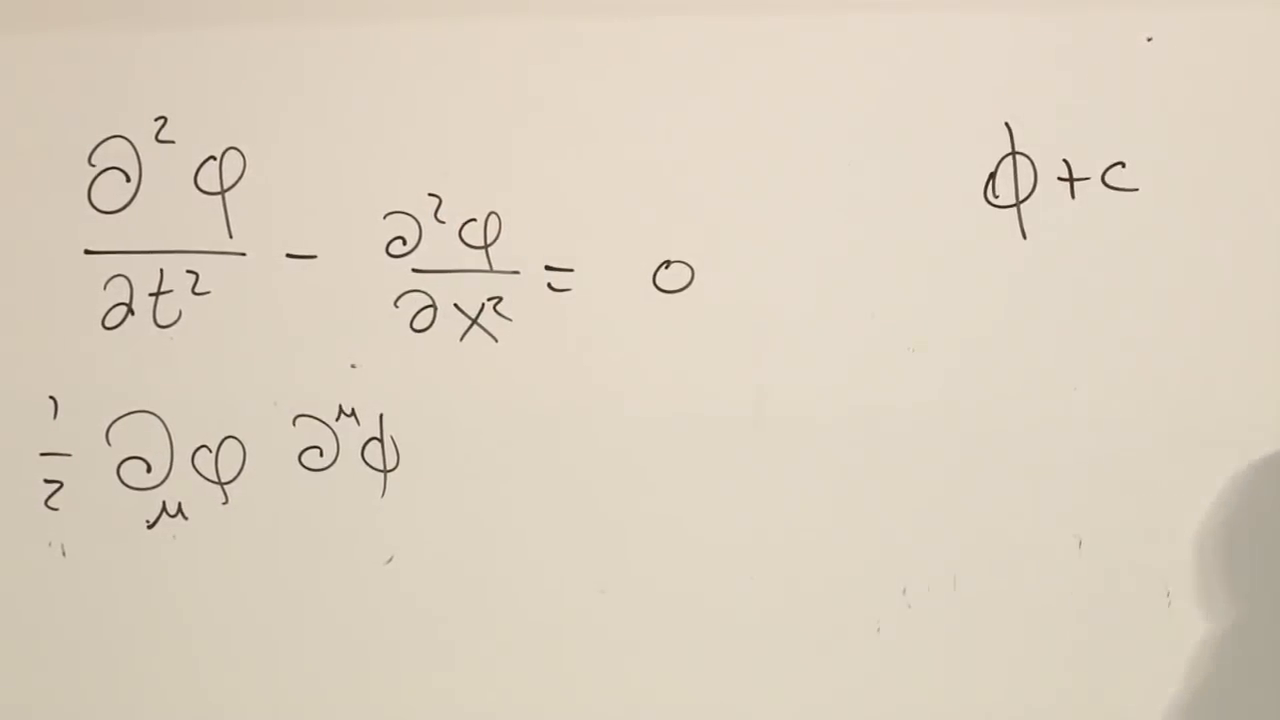
\includegraphics[width=0.90\textwidth]{lecture_07_figure_17.png}
\caption{无质量波动方程、其导数拉格朗日量以及常数平移 \(\phi\mapsto\phi+c\)。}
\lectureframe{01:17:10}
\end{figure}

现在加入质量项：
\begin{equation}
\frac{\partial^2\phi}{\partial t^2}
-\frac{\partial^2\phi}{\partial x^2}
+\mu^2\phi
=0,
\end{equation}
\begin{equation}
\mathcal L_\mu
=
-\frac12\partial_\mu\phi\,\partial^\mu\phi
-\frac{\mu^2}{2}\phi^2.
\label{eq:sr7-massive-L}
\end{equation}
导数部分在
\(\phi\mapsto\phi+c\) 下保持不变，但 \(\phi^2\) 不是。两种理论都是合法的；一种具有平移不变性，另一种则没有。

\begin{figure}[htbp]
\centering
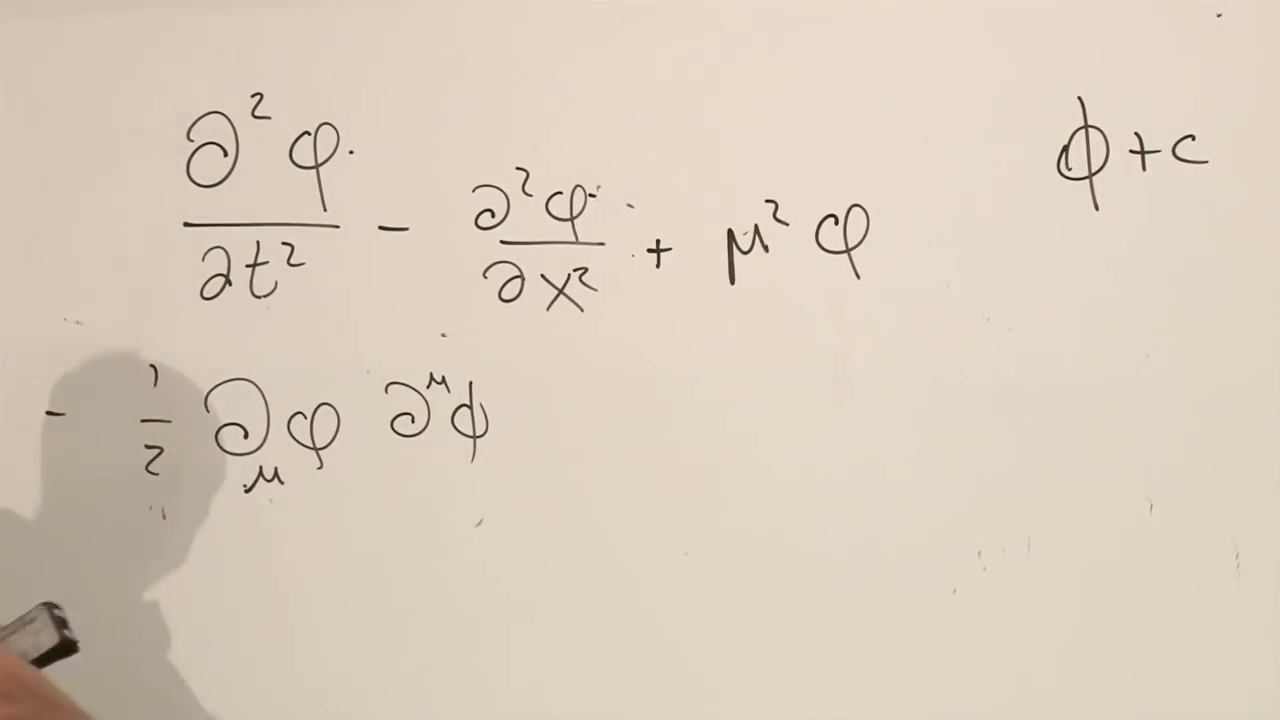
\includegraphics[width=0.90\textwidth]{lecture_07_figure_18.png}
\caption{破坏常数平移不变性的质量项。}
\lectureframe{01:18:50}
\end{figure}

\subsection{一名学生预见到边界项}

一位听众提出了一个更严格的检验：
\begin{equation}
\phi(x,t)\longrightarrow\phi(x,t)+x.
\label{eq:sr7-linear-shift}
\end{equation}
\(x\) 的二阶导数为零，因此无质量波动方程仍然满足。作用量需要更仔细地考察。由于 \(x\) 和 \(t\) 是独立变量，
\begin{equation}
\frac{\partial x}{\partial t}=0,
\qquad
\frac{\partial x}{\partial x}=1.
\end{equation}
空间部分按照下式变化
\begin{align}
-\frac12
\left[
\partial_x(\phi+x)
\right]^2
&=
-\frac12
\left(
\partial_x\phi+1
\right)^2
\notag\\
&=
-\frac12(\partial_x\phi)^2
-\partial_x\phi
-\frac12.
\label{eq:sr7-linear-shift-L}
\end{align}
新增的项是一个常数和一个全导数。常数不改变欧拉--拉格朗日方程。对
\(\partial_x\phi\) 积分只产生空间边界值，因此在通常的固定边界条件下，它也不改变运动方程。

\begin{figure}[htbp]
\centering
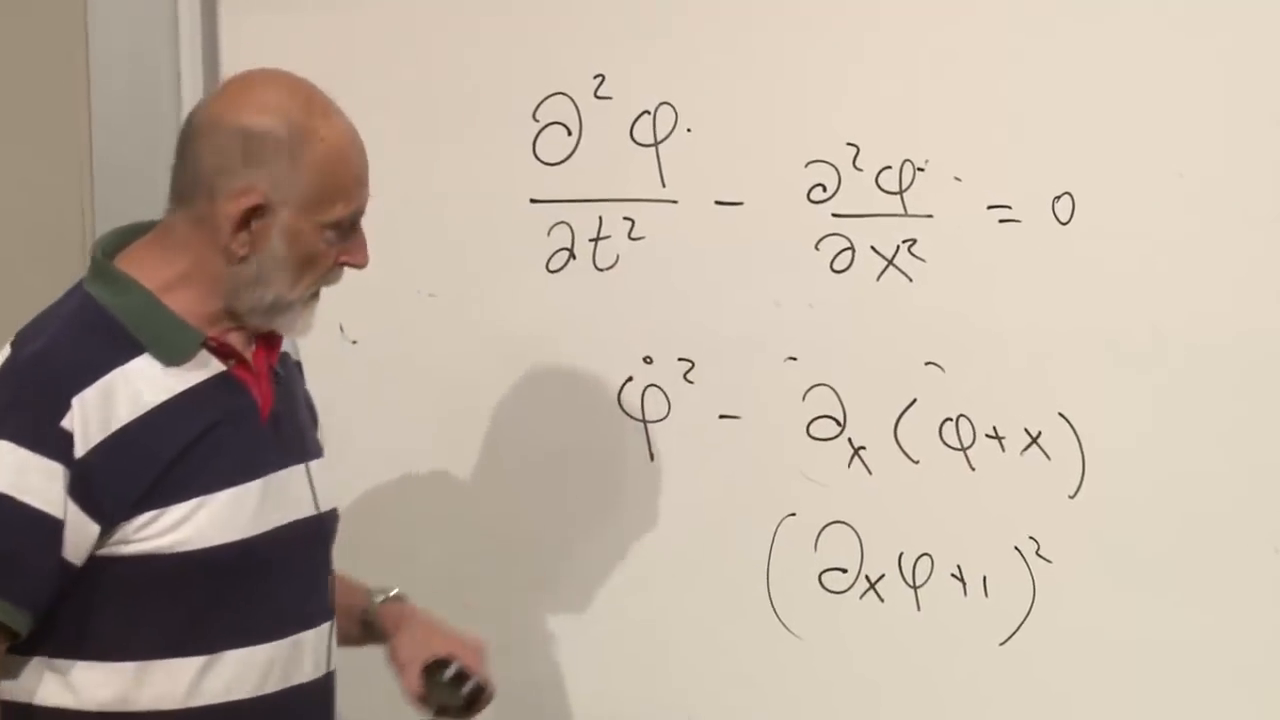
\includegraphics[width=0.90\textwidth]{lecture_07_figure_19.png}
\caption{所提出的平移 \(\phi\mapsto\phi+x\) 以及揭示出一个常数加一个全导数的导数平方。}
\lectureframe{01:22:40}
\end{figure}

\begin{classroomqa}
\audiencequestion{尽管 \(\phi\mapsto\phi+x\) 改变了拉格朗日密度，它是否保持无质量场方程不变？}
\lecturerresponse{是的。\(x\) 的二阶导数为零，因此方程不变。拉格朗日量只改变一个常数和一个空间全导数。这些项使作用量的数值改变一个固定的体常数和边界值，但在固定边界条件下不改变欧拉--拉格朗日方程。\lecturetimestamp{01:20:00}}
\end{classroomqa}

\begin{classroomqa}
\audiencequestion{为什么 \(\partial x/\partial t\) 为零？}
\lecturerresponse{因为 \(x\) 和 \(t\) 是场描述中的独立坐标。对 \(t\) 的偏导数保持
\(x\) 固定。\lecturetimestamp{01:22:22}}
\end{classroomqa}

这名学生已经得到了电磁学所需的工具：一个全导数可以改变写出的作用量，而不改变其驻定路径。

\section{带电粒子的规范不变性}

\subsection{添加一个四维梯度}

回到相互作用
\begin{equation}
I_{\mathrm{int}}
=
-e\int A_\mu\,dx^\mu.
\end{equation}
设 \(\Lambda(x)\) 为任意足够光滑的标量，并将势改变为
\begin{equation}
A_\mu
\longrightarrow
A'_\mu
=
A_\mu+\partial_\mu\Lambda.
\label{eq:sr7-gauge-transformation}
\end{equation}
梯度 \(\partial_\mu\Lambda\) 与 \(A_\mu\) 具有相同的协变指标结构，因此该和是良定义的。

\begin{figure}[htbp]
\centering
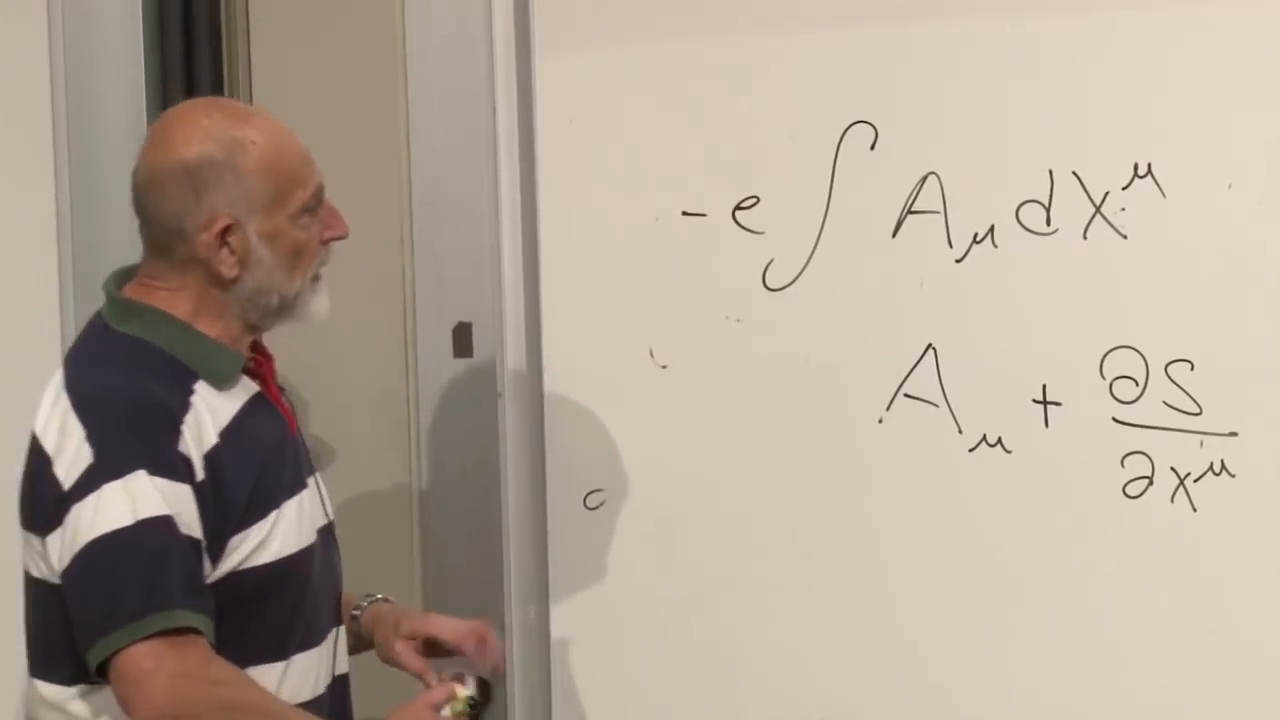
\includegraphics[width=0.90\textwidth]{lecture_07_figure_20.png}
\caption{世界线耦合与变换 \(A_\mu\mapsto A_\mu+\partial_\mu\Lambda\)。}
\lectureframe{01:24:50}
\end{figure}

作用量的改变为
\begin{align}
\Delta I_{\mathrm{int}}
&=
-e\int \partial_\mu\Lambda\,dx^\mu
\notag\\
&=
-e\int d\Lambda
\notag\\
&=
-e\left[
\Lambda(x_2)-\Lambda(x_1)
\right].
\label{eq:sr7-gauge-boundary}
\end{align}
沿每一无穷小世界线段，\(\partial_\mu\Lambda\,dx^\mu\) 恰好就是增量 \(d\Lambda\)。将这些增量相加便望远镜式地化为终点值与起点值之差。

\begin{figure}[htbp]
\centering
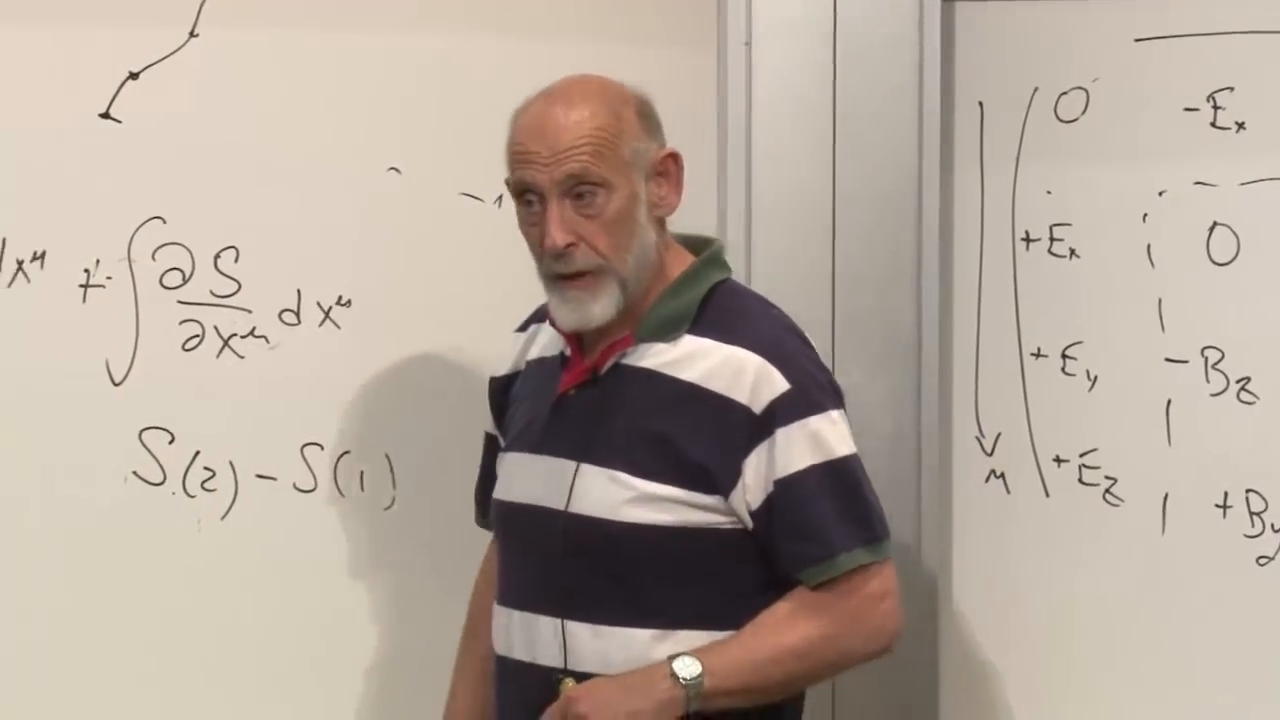
\includegraphics[width=0.90\textwidth]{lecture_07_figure_21.png}
\caption{梯度贡献沿路径积分后成为端点差 \(\Lambda(x_2)-\Lambda(x_1)\)。}
\lectureframe{01:28:10}
\end{figure}

变分原理比较的是 \(x_1\) 与 \(x_2\) 保持固定的邻近轨道。因此 \eqref{eq:sr7-gauge-boundary} 中的额外项对每一种允许的变分都相同：
\begin{equation}
\delta\Delta I_{\mathrm{int}}=0.
\end{equation}
稳定轨道不变。这就是作为端点陈述的规范不变性。

\begin{classroomqa}
\audiencequestion{\(\Lambda\) 可以是任意标量函数吗？}
\lecturerresponse{可以，但须满足导数和作用量所需的平滑性与边界假设。该变换是局域的，因为参数是时空的任意函数，而不仅仅是一个整体常数。\lecturetimestamp{01:28:40}}
\end{classroomqa}

给 \(A_\mu\) 加上一个梯度称为规范变换。规范一词是历史遗留；讲座以幽默而坚定的方式告诫，不要把它读得像一个法语词。名称不如运算本身重要。

\subsection{用场张量直接证明}

运动方程依赖于 \(F_{\mu\nu}\)，而不依赖于势本身。在 \eqref{eq:sr7-gauge-transformation} 下，
\begin{align}
F'_{\mu\nu}
&=
\partial_\mu
\left(
A_\nu+\partial_\nu\Lambda
\right)
-
\partial_\nu
\left(
A_\mu+\partial_\mu\Lambda
\right)
\notag\\
&=
F_{\mu\nu}
+
\partial_\mu\partial_\nu\Lambda
-
\partial_\nu\partial_\mu\Lambda
\notag\\
&=
F_{\mu\nu}.
\label{eq:sr7-F-gauge-invariant}
\end{align}
对于普通平坦时空中的光滑标量，偏导数可交换。两个额外项相消。因此场张量、它所包含的电场和磁场，以及力定律，全都是规范不变的。

\begin{figure}[htbp]
\centering
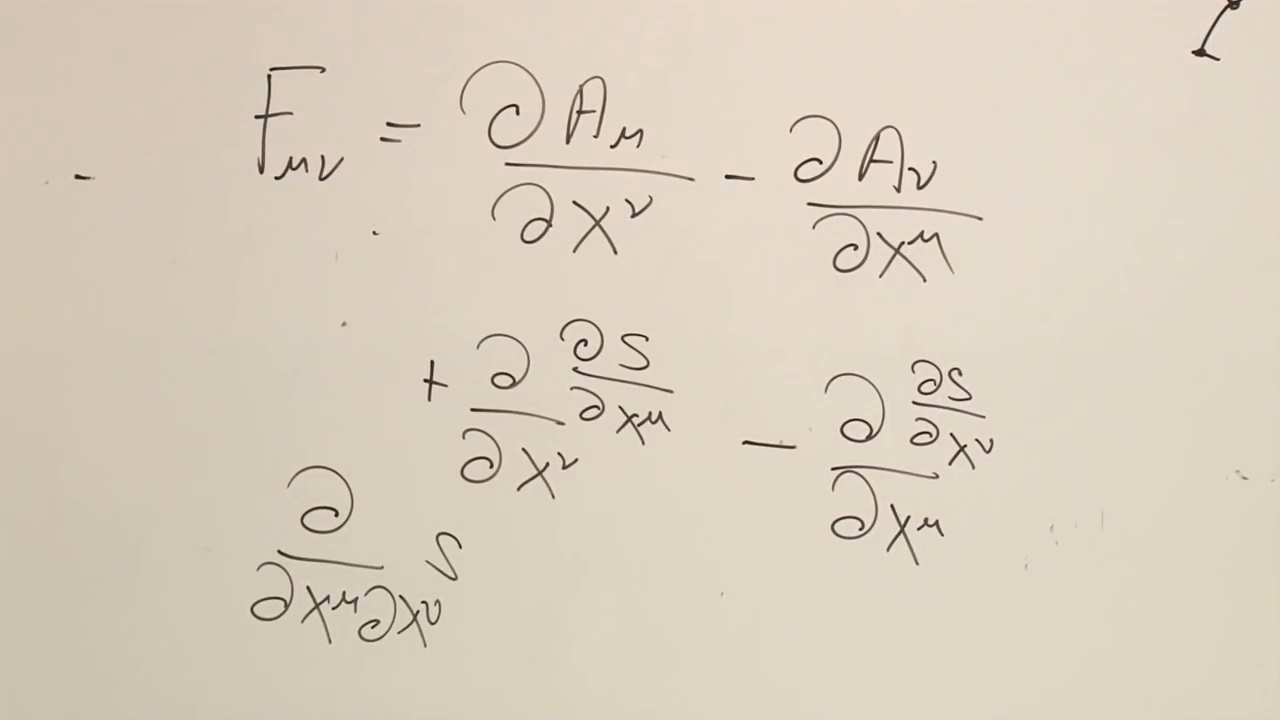
\includegraphics[width=0.90\textwidth]{lecture_07_figure_22.png}
\caption{由规范变换产生的两个二阶导数相消，因为偏导数可交换。}
\lectureframe{01:33:50}
\end{figure}

这两个证明从相反方向闭合了同一个循环。作用量只在固定端点处改变，而方程只依赖于未改变的场张量。

\section{冗余意味着什么}

\subsection{为什么要保留一个不唯一的对象？}

自然的反对意见立刻出现。如果 \(A_\mu\) 不唯一，我们为什么要引入它？因为它对局域洛伦兹不变作用量不可或缺，尽管其分量值包含冗余信息。许多势表示同一个电磁场：
\begin{equation}
A_\mu
\sim
A_\mu+\partial_\mu\Lambda.
\end{equation}
等价类是物理的；某个特定代表元是一种描述的选择。

\begin{classroomqa}
\audiencequestion{改变规范有实际价值吗？}
\lecturerresponse{有。适当的 \(\Lambda\) 可以简化势的某个分量，或使问题的某个特征变得透明。在局域且边界条件适当时，人们常常可以选择一种规范，使某个选定的分量，包括 \(A_0\)，为零。另一种规范可能更清楚地显示另一个特征。\lecturetimestamp{01:35:43}}
\end{classroomqa}

\begin{classroomqa}
\audiencequestion{规范不变性是否类似于从两个洛伦兹参考系描述同一个实验？}
\lecturerresponse{不。洛伦兹变换比较的是不同观测者所携带的物理上有意义的参考系。规范变换是同一种描述内部的冗余：不同的势编码同一个场。数学上两者都是不变性，但它们的解释不同。\lecturetimestamp{01:37:07}}
\end{classroomqa}

还有一个结构上的区别。旋转使用一个固定的整体角度；人们通常不会在每一点用互不相关的角度旋转坐标轴。规范变换由整个函数 \(\Lambda(x)\) 参数化。正是这种依赖于位置的自由度使它成为局域规范不变性。

\begin{classroomqa}
\audiencequestion{加上一个梯度是规范不变性的一般定义吗？}
\lecturerresponse{对于阿贝尔电磁理论，那就是该变换。杨--米尔斯理论有一个更复杂的非阿贝尔版本，其中势带有额外的内部结构，但同样的思想仍然成立：不同的局域描述表示相同的物理。\lecturetimestamp{01:39:27}}
\end{classroomqa}

\begin{classroomqa}
\audiencequestion{规范变换仅仅是一种数学手段，用来突出问题的不同部分吗？}
\lecturerresponse{它是一种有用的计算和解释手段，但其作用受到约束：它可以简化方程或揭示某种性质，却不能改变任何最终的规范不变预言。
\lecturetimestamp{01:40:22}}
\end{classroomqa}

\subsection{其他场与其他势}

其他理论中的规范势通常也用\(A\)表示，并带有时空指标\(\mu\)。它们的不同之处在于与其他对称性相关的额外内部结构。本讲推迟讨论这一结构，而不是给出一个过早的公式。

\begin{classroomqa}
\audiencequestion{其他场论的矢量势是什么样子的？}
\lecturerresponse{它们仍然表现为时空矢量，通常写作\(A_\mu\)，但带有与内部对称性相关的额外标签和代数结构。这就是通往Yang--Mills理论的入口，此处有意推迟讨论。\lecturetimestamp{01:41:02}}
\end{classroomqa}

\begin{classroomqa}
\audiencequestion{真的不可能直接用\(\mathbf E\)和\(\mathbf B\)写出局域洛伦兹不变的带电粒子作用量吗？}
\lecturerresponse{在此处陈述的假设范围内，是的。本讲将其作为一条定理提出，但并未证明它。保持作用量原理、局域性和洛伦兹不变性会迫使引入势，此后规范冗余便自动出现。
\lecturetimestamp{01:42:18}}
\end{classroomqa}

\subsection{什么可以被测量？}

\(A_\mu\)的局域值本身不是规范不变的。如果一次物理测量唯一地确定了该值，那么将其改变\(\partial_\mu\Lambda\)就会改变一个物理结果，这与刚刚证明的不变性相矛盾。可测量的预言必须由规范不变量构成，例如在当前经典讨论中的\(F_{\mu\nu}\)。

\begin{classroomqa}
\audiencequestion{为什么自然界如此执着地选择规范理论？}
\lecturerresponse{在经典层面，本讲没有给出最终理由。量子力学提供了更深刻的视角，但即便在那里，宽泛的答案也未被穷尽。已经显而易见的是，由规范冗余组织起来的理论具有不寻常的美、对称性和经济性。
\lecturetimestamp{01:43:36}}
\end{classroomqa}

\begin{classroomqa}
\audiencequestion{矢量势本身可以被测量吗？}
\lecturerresponse{不能作为依赖规范的局域分量值来测量。测量是一个物理过程，而每一个物理预言都必须对\(A_\mu\mapsto A_\mu+\partial_\mu\Lambda\)不敏感。可以被测量的是势和场的规范不变特征。
\lecturetimestamp{01:44:18}}
\end{classroomqa}

\begin{classroomqa}
\audiencequestion{如果\(A_\mu\)被某个不是梯度的东西改变，会发生什么？}
\lecturerresponse{一般而言\(F_{\mu\nu}\)会改变，因此这种改变是可探测的。相比之下，纯规范势\(A_\mu=\partial_\mu\Lambda\)有\(F_{\mu\nu}=0\)，不施加任何电磁力；此时自由粒子沿直线世界线运动。\lecturetimestamp{01:45:22}}
\end{classroomqa}

因此，规范不变性不是一种可以随意丢弃的技巧。电动力学、Yang--Mills理论、标准模型和引力都具有某种或另一种规范冗余。这种模式很奇特：为了表述理论，需要一个辅助量，但该量的一部分可以在不改变物理的情况下被改变。这种奇特之处也正是其组织力量之所在。

\section{规范不变性的逻辑}

本讲走了一条刻意迂回的道路。我们首先恢复了上--下指标语言，因为标量缩并是洛伦兹不变作用量的语法。然后我们陈述了四条原理：作用量、局域性、洛伦兹不变性和规范不变性。在重建带电粒子计算的过程中，第四条一直未被定义。

该计算从局域标量作用量
\begin{equation}
I
=
-m\int d\tau
-e\int A_\mu dx^\mu,
\end{equation}
出发，经过普通时间拉格朗日量和每一个Euler--Lagrange导数，恢复了电和磁的洛伦兹力。然后固有时将结果组装成
\begin{equation}
m\frac{du^\mu}{d\tau}
=
-eF^\mu{}_\nu u^\nu,
\qquad
F_{\mu\nu}
=
\partial_\mu A_\nu-\partial_\nu A_\mu.
\end{equation}

标量场的例子为最后一步做了准备：全导数只能通过边界改变作用量。因此，
\begin{equation}
A_\mu\longrightarrow A_\mu+\partial_\mu\Lambda
\end{equation}
只通过固定的端点值改变世界线作用量，并且由于混合偏导数可交换而保持\(F_{\mu\nu}\)不变。因此，矢量势是必要的，但不是唯一的。规范不变性所陈述的是：这种不唯一性属于描述，而不属于物理。
